\section{Modelo de Datos}

Un modelo de datos tiene el propósito de proveer el detalle de la definición de la estructura de la información que será gestionada en el repositorio en términos de tipos de datos, relaciones y organización. Para el caso del proceso de finanzas (Cuentas Contables) se construyeron los siguientes modelos de datos:

\subsection{[CuCo] Cuentas Contables}

Modelo que contiene la información de las cuentas contables creadas. Dentro del modelo se encuentran creadas 9 tablas/entidades:
\begin{enumerate}
    \item \textbf{Cuenta maestra (Mandante):}
    Tabla que contiene la información de las cuentas contables que han sido creadas, así como las que han sido modificadas o bloqueadas, provenientes de SAP.
    
    \item \textbf{Cuenta maestra (Descripción):}
    Tabla que contiene la información de las descripciones y tipo de idioma de las cuentas provenientes de SAP.

    \item \textbf{Cuenta maestra (Sociedad):}
    Tabla que contiene todas las cuentas asociadas a una sociedad que proviene de SAP.
    
    \item \textbf{[EBX] Base de Cuenta maestra}
    Tabla auxiliar que contiene la información de cuentas contables creadas, modificadas o bloqueadas, sin ser ampliadas.
    
    \item \textbf{[EBX] Base de Cuenta maestra – Sociedad}
    Tabla auxiliar que contiene la información de cuentas contables creadas, modificadas o bloqueadas, al ser ampliadas.
    
    \item \textbf{[EBX] Sociedad – Cuenta Maestra}
    Tabla auxiliar que contiene los registros individuales de aquellas cuentas asociadas a una sociedad.
    
    \item \textbf{[EBX] Creación cuenta multimandante}
    Tabla auxiliar que contiene la información general de una cuenta multimandante.
    
    \item \textbf{[EBX] Unidad – Cuenta multimandante}
    Tabla auxiliar que contiene los registros específicos creados para una cuenta multimandante dividido por mandantes.
    
    \item \textbf{[EBX] Carga Masiva – PUC}

    Tabla auxiliar para crear solicitudes de carga masiva a nivel PUC.

    \item \textbf{[EBX] Carga Masiva – Sociedad}

    Tabla auxiliar para crear solicitudes de carga masiva a nivel PUC.

    \item \textbf{[Masiva] Nivel PUC}

    Tabla auxiliar donde se pre cargan las cuentas a procesar en una carga masiva a nivel PUC.

    \item \textbf{[Masiva] Sociedad}

    Tabla auxiliar donde se pre cargan las cuentas y sociedades a procesar en una carga masiva a nivel Sociedad.
\end{enumerate}

\begin{figure}[H]
    \centering
    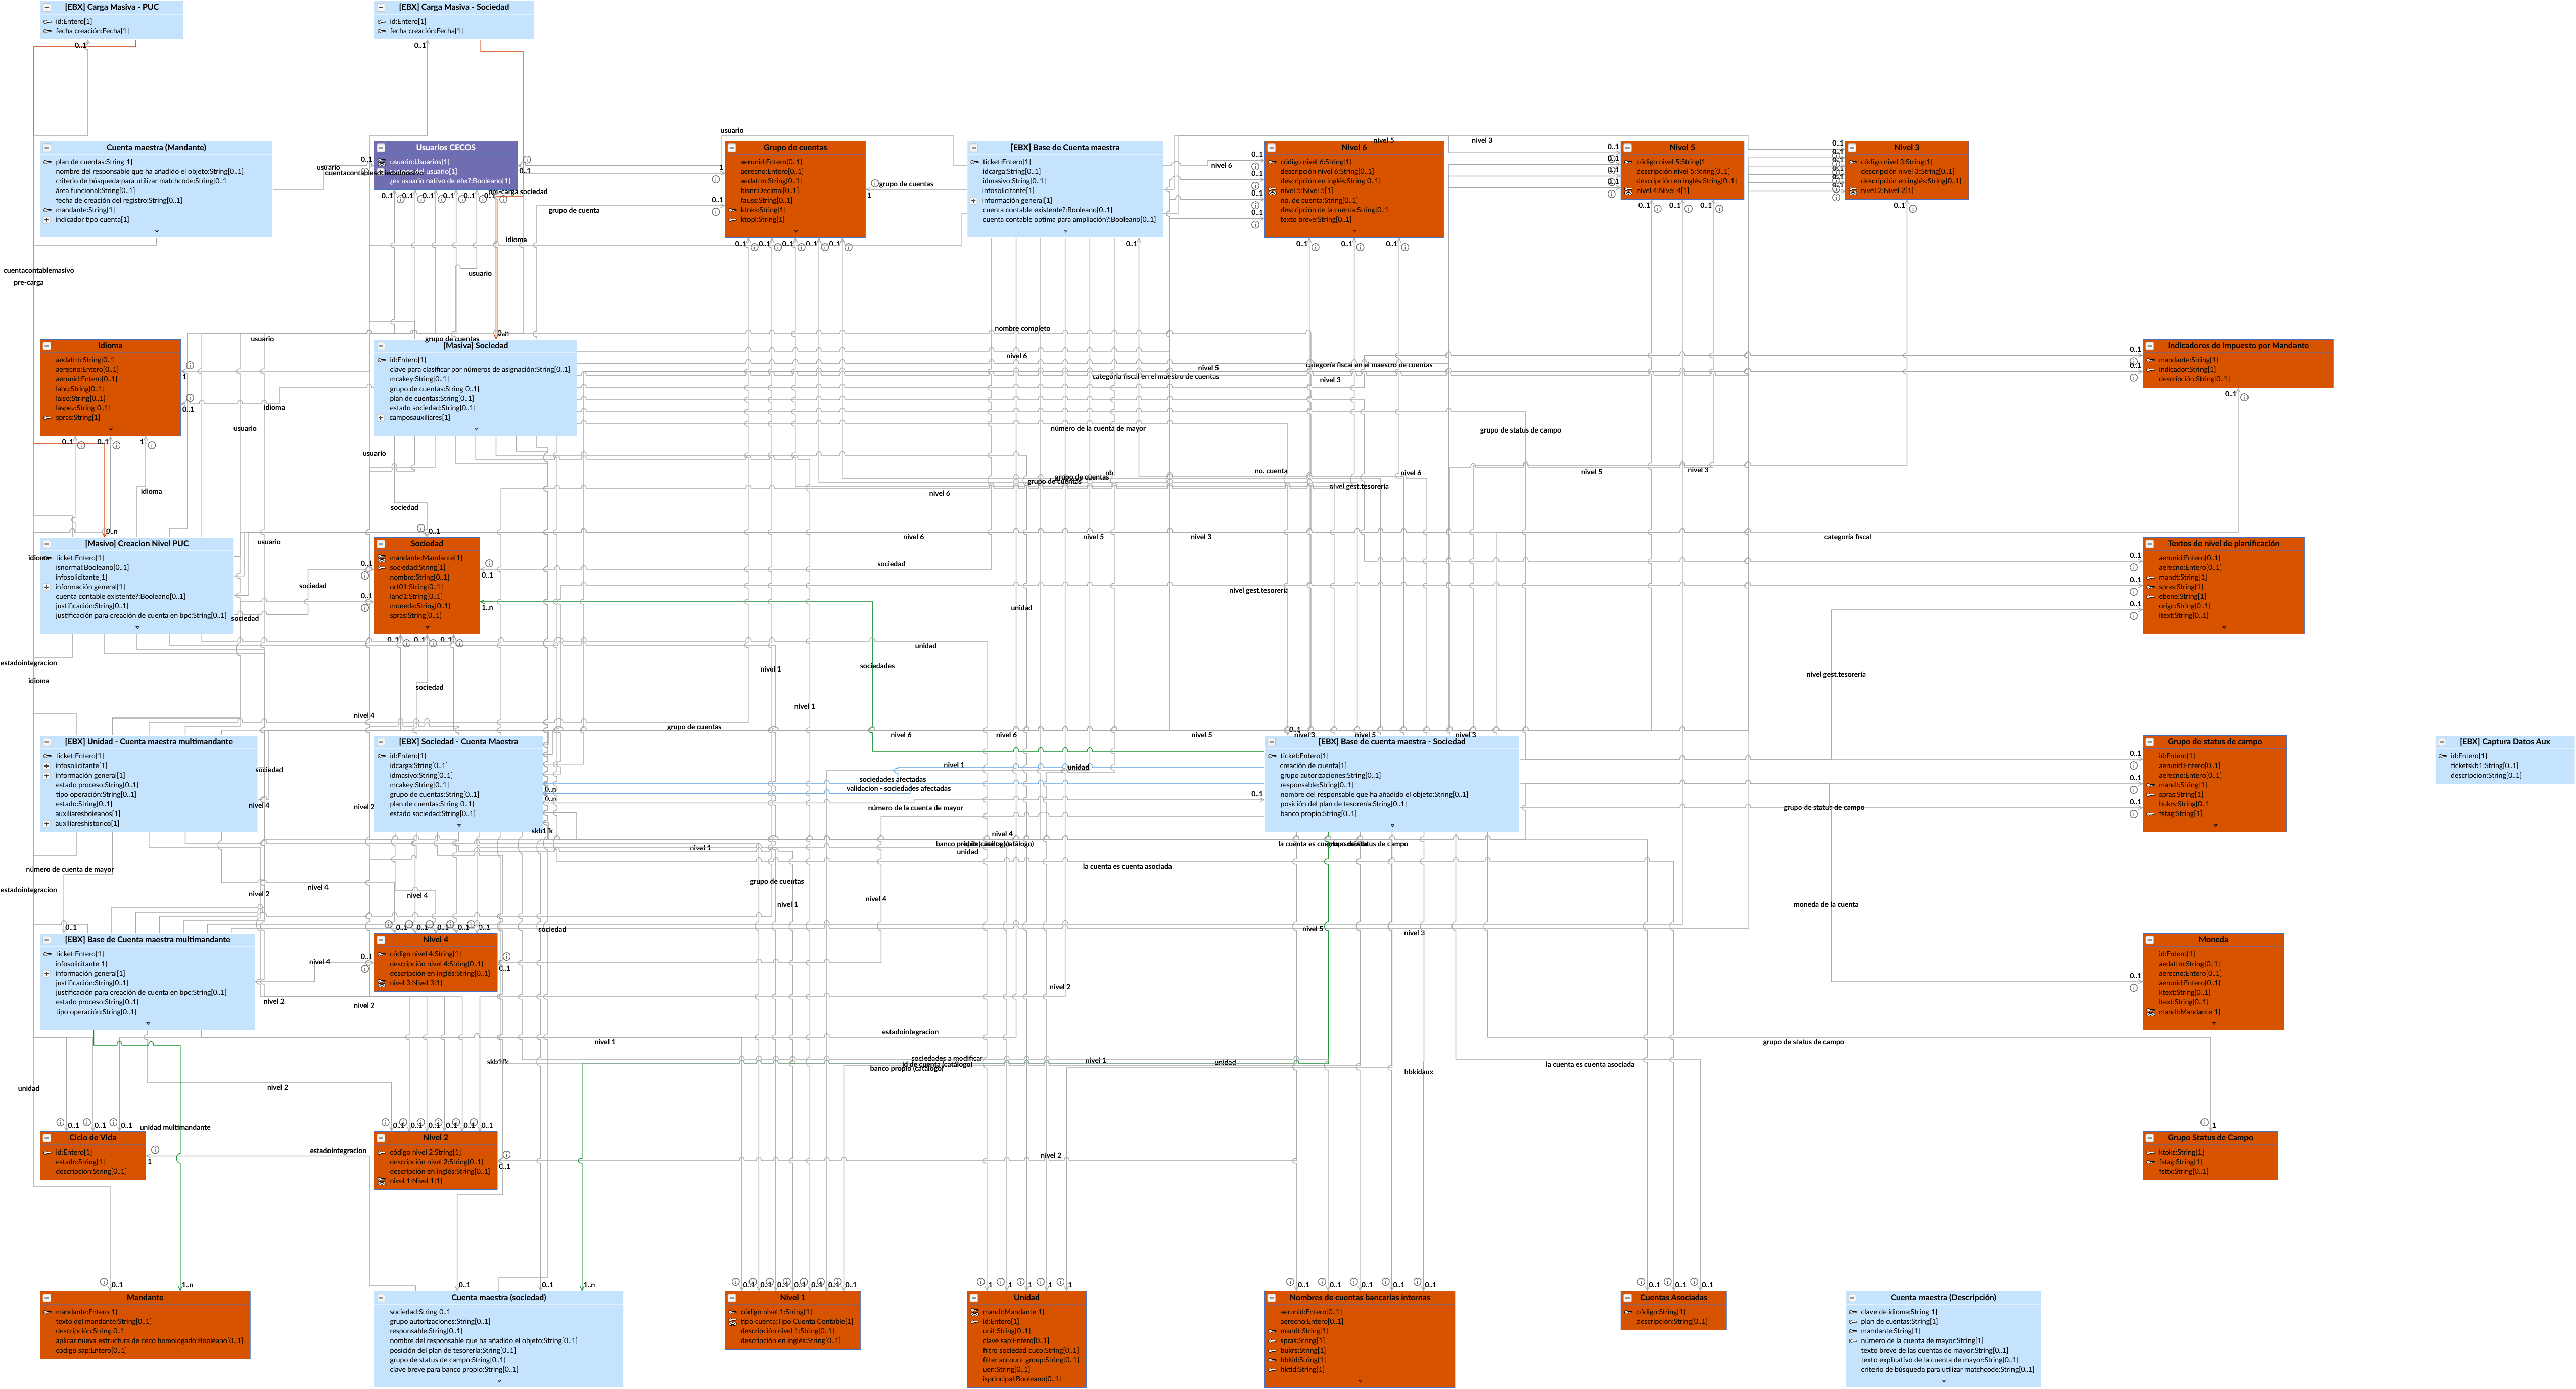
\includegraphics[width=0.8\textwidth]{ModeloDatos/ImagenesModelosDatos/CuentasContablesNuevo.png}
    \caption{Diagrama del modelo de datos de Cuentas Contables}
\end{figure}%


\begin{quote}
  \textbf{Nota:} Para mejor calidad se adjuntan imágenes de los diagramas en el correo.
\end{quote}


%% ------ Calidad------
\subsection{[CuCo] Cuentas Contables – Calidad}

Modelo diseñado para contener la información a la cual se le aplicarán las distintas reglas de calidad, para este proceso se hizo uso de 3 tablas/entidades:

\begin{enumerate}
         \item SKA1:
        Tabla auxiliar que contiene las cuentas contables pertenecientes a SAP, más un apartado para el cálculo de reglas backend de cuentas contables.
        \item SKAT:
        Tabla auxiliar que contiene las descripciones cuentas contables pertenecientes a SAP, más un apartado para el cálculo de reglas backend de cuentas contables.
        \item SKB1: 
        Tabla auxiliar que contiene las cuentas contables asociadas a una sociedad pertenecientes a SAP, más un apartado para el cálculo de reglas backend de cuentas contables.
\end{enumerate}

%% ####### landing

\subsection{Cuentas Contables Landing}

Espacio de aterrizaje de los datos pertenecientes a SAP.

\begin{enumerate}
         \item SKA1:
        Tabla auxiliar que contiene las cuentas contables pertenecientes a SAP.
        \item SKAT:
        Tabla auxiliar que contiene las descripciones cuentas contables pertenecientes a SAP.
        \item SKB1: 
        Tabla auxiliar que contiene las cuentas contables asociadas a una sociedad pertenecientes a SAP.
\end{enumerate}


%% ################ CA ##########

\subsection{[CA] Customized Administration}

Modelo auxiliar para llevar a cabo la integración, principalmente se hace uso de la entidad/tabla “Monitoreo EBX”, la cual se compone de lo siguiente:
\begin{itemize}
    \item \textbf{Estado:}  Contiene los estados en lo que se encuentra la integración, los cuales pueden ser pre-carga, esperando respuesta, erróneo, invalida, completado e inexistente. 
    
    \item \textbf{Mapeo:} Contiene la configuración pertinente para un mapeo de los campos de una tabla de EBX hacia una estructura JSON.
    
    \item \textbf{Parámetros Encabezados:} Contiene los parámetros ligados a la cabecera de una petición REST.
    
    \item \textbf{Parámetros de Consulta:} Parámetros de consulta del servicio web.
    
    \item \textbf{Request Workflow State:}  Contiene una bitácora de las solicitudes generadas a lo largo del tiempo.
    
    \item \textbf{Configuración del Workflow – Estado:} Contiene la relación entre el flujo de trabajo ejecutado con el estado en el que el ente se encuentra.
\end{itemize}

Dentro el proceso de carga masiva se hace uso de la entidad/tabla \textbf{WFMasivo}
\begin{itemize}
    \item \textbf{Pasos;} listado de pasos a seguir en el flujo masivo es este caso el listado de validadores
    \item \textbf{Condicionales:} listado de condiciones para permanecer en el paso actual, dentro de cuentas es el listado de condiciones y asignaciones de variables para el validador actual continué o asigne el flujo de trabajo.
\end{itemize}

\begin{figure}[H]
    \centering
    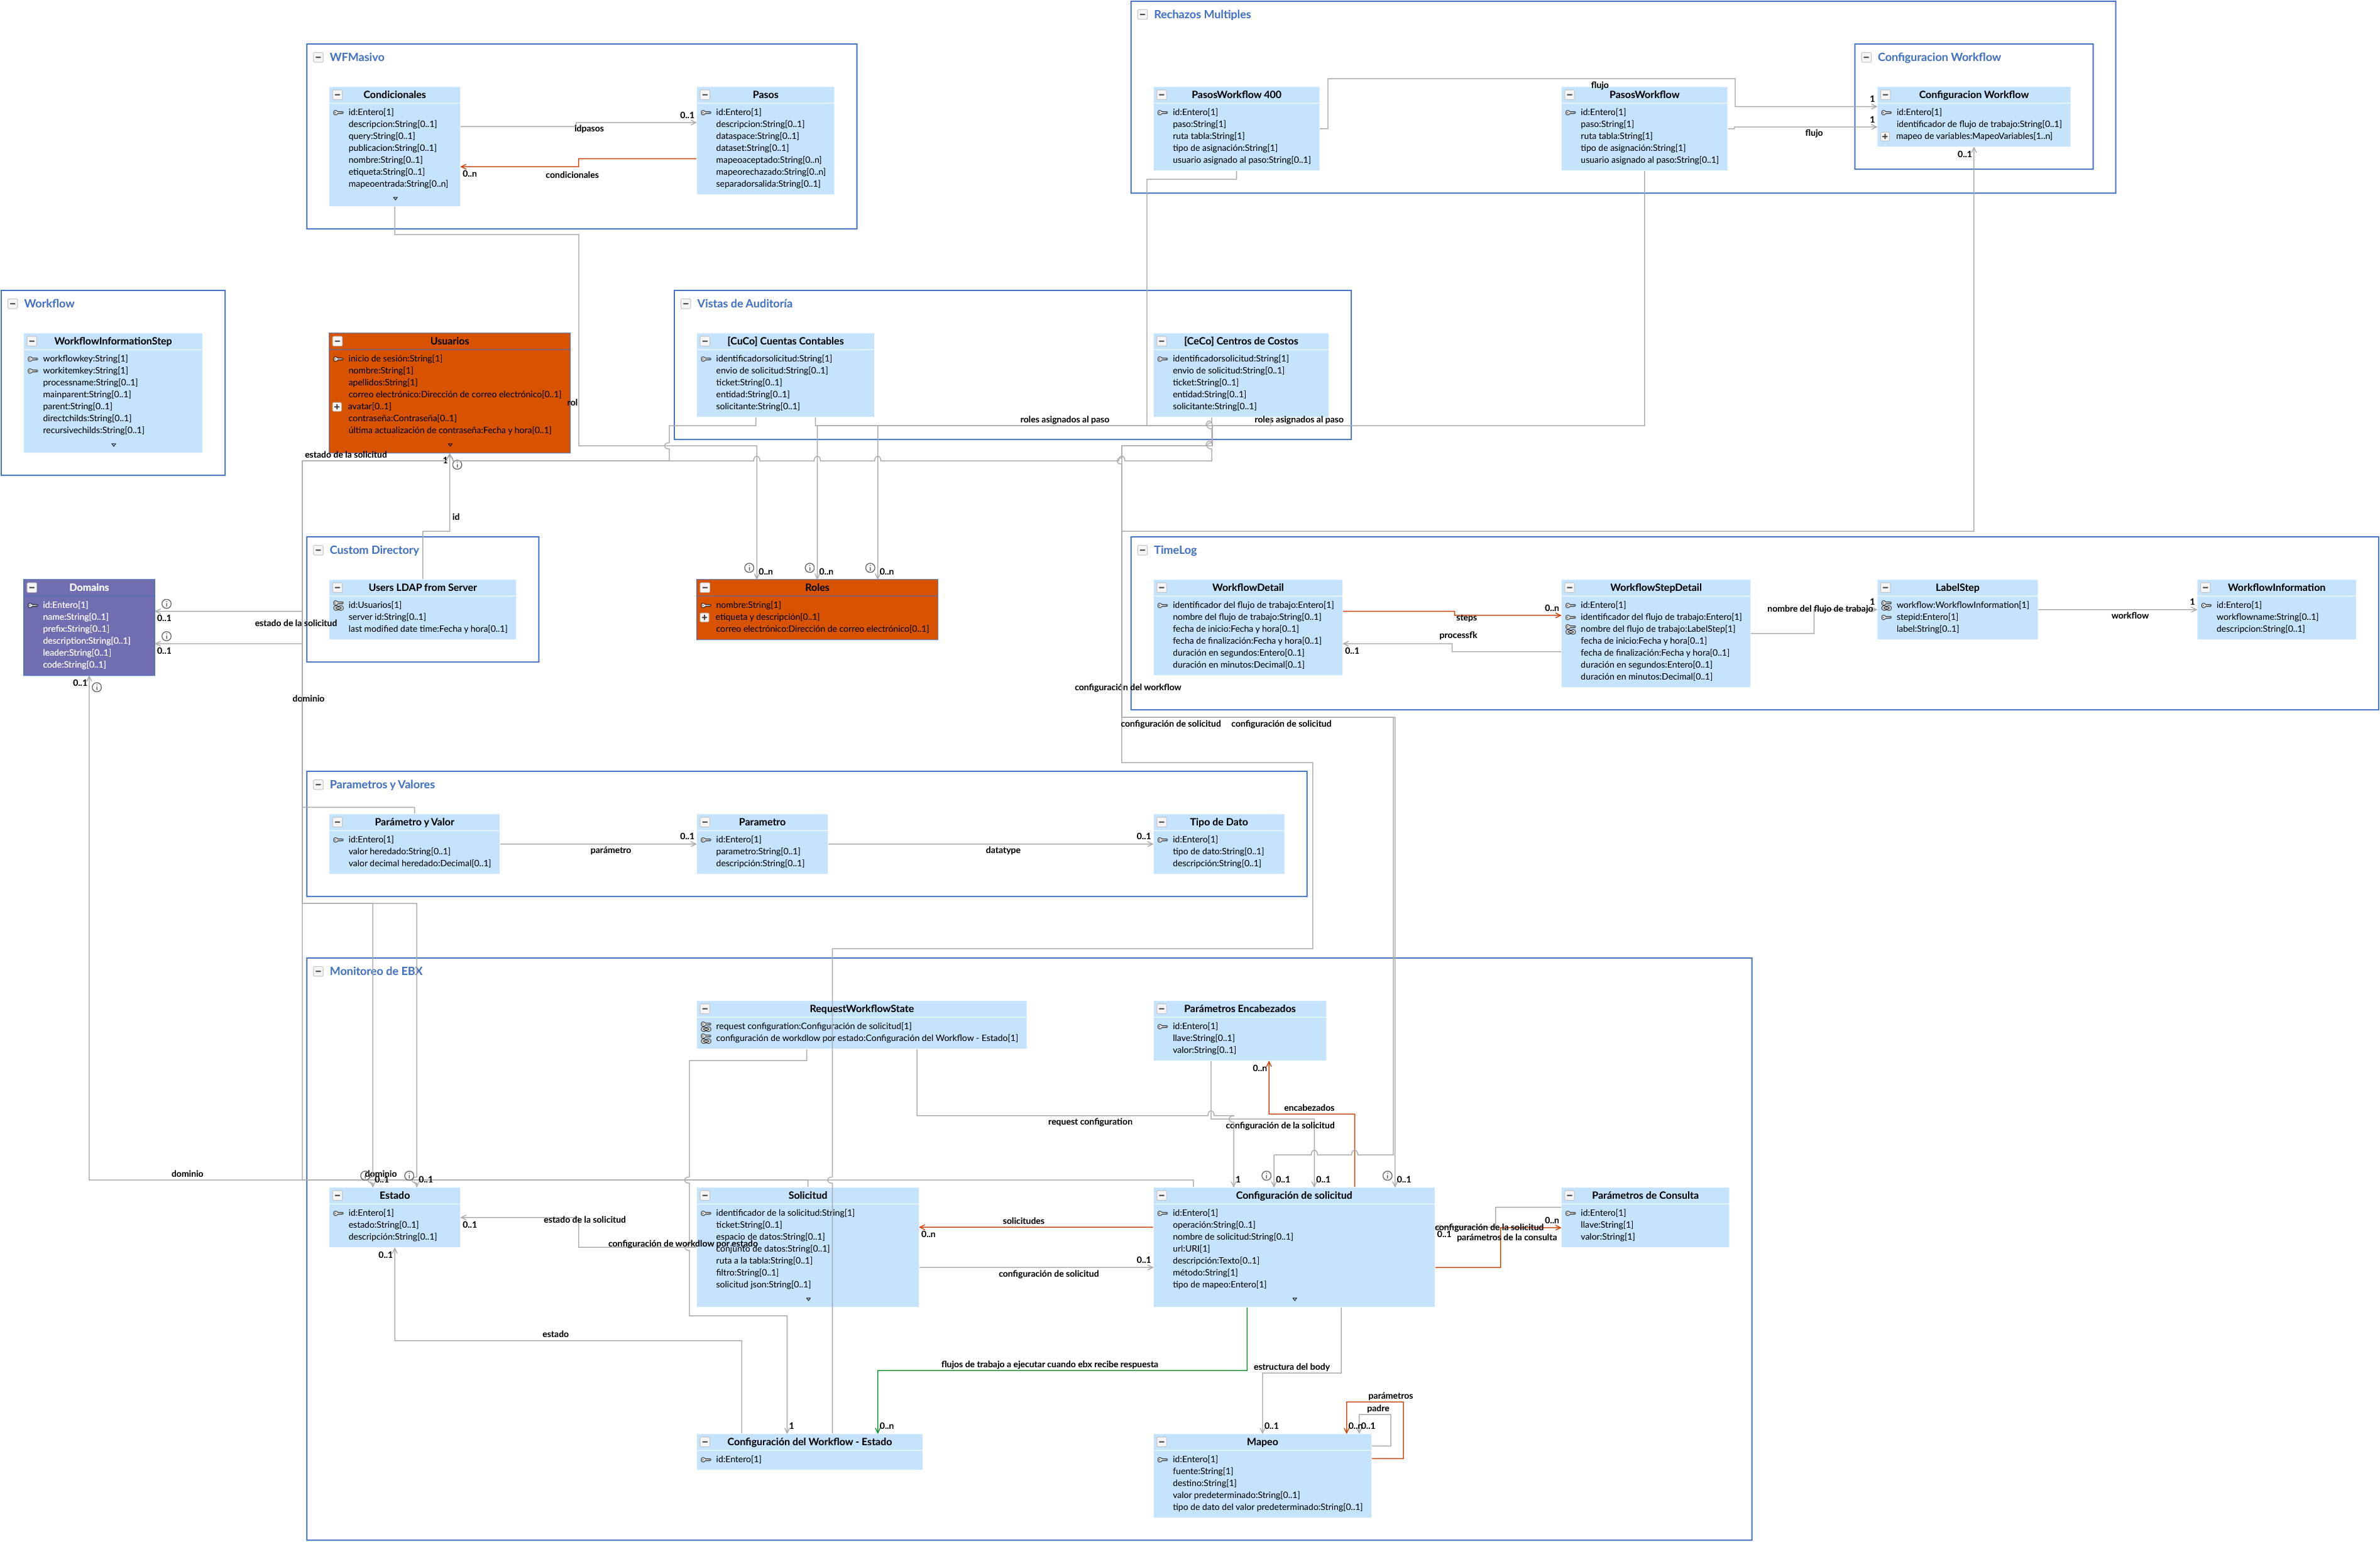
\includegraphics[width=0.8\textwidth]{ModeloDatos/ImagenesModelosDatos/CustomizedAdministration.png}
    \caption{Diagrama del modelo de datos del catálogo de Customized Administration}
\end{figure}


\begin{quote}
  \textbf{Nota:} Para mejor calidad se adjuntan imágenes de los diagramas en el correo.
\end{quote}

%%%%%%%%%%% [CA] Catálogos Maestros}
\subsection{[CA] Catálogos Maestros}

Contiene distintas tablas, las cuales se utilizan como un punto de referencia a la información de la organización para un camino optimo en el proceso relevante.

{\centering
\textbf{Cuentas Contables}\par}

\begin{enumerate}

    \item Grupo de cuentas: Catálogo de distribución de los diferentes grupos de cuentas (cuentas de mayor) admitidas en el proceso.
    
    \item Plan de cuentas: Catálogo de los diferentes planes de cuentas admitidos durante el proceso.
    
    \item Grupo de status de campo: Catálogo de distribución de las denominaciones de los diferentes grupos de status de campos.
    
    \item Textos de nivel de planificación: Catálogo de distribución de los textos en base a los niveles de tesorería.
    
    \item Nombres de cuentas bancarias internas: Catálogo de distribución con las cuentas de bancos propios.

    \item Idioma: Catálogo de distribución de los diferentes posibles idiomas utilizados en los procesos de CMI.

    \item Tipo de cuentas contables: Catálogo de distribución de los tipos de cuentas que pueden crearse.

    \item Indicadores de impuesto por mandante: Catálogo de distribución asociado al campo “Categoría fiscal en el maestro de cuentas” en procesos a nivel Sociedad.

    \item Cuentas Asociadas: Catálogo de distribución asociado al campo “La cuenta es cuenta asociada” en procesos a nivel Sociedad.

    \item Nivel Cuentas
    \begin{enumerate}
        \item Nivel 1: 
        Catalogo funcional que contiene la información del primer nivel de una cuenta contable, este catálogo depende del tipo de Banco.
        \item Nivel 2:
        Catalogo funcional que contiene la información del segundo nivel de una cuenta contable, este espacio depende del primer nivel.
        \item Nivel 3: 
        Catalogo funcional que contiene la información del tercer nivel de una cuenta contable, este espacio depende del segundo nivel.
        \item Nivel 4:
        Catalogo funcional que contiene la información del cuarto nivel de una cuenta contable, este espacio depende del tercer nivel.
        \item Nivel 5:
        Catalogo funcional que contiene la información del quinto nivel de una cuenta contable, este espacio depende del cuarto nivel.
        \item Nivel 6:
        Catalogo funcional que contiene la información del sexto nivel de una cuenta contable, este espacio depende del quinto nivel; además de contener la descripción de la cuenta y cuenta alternativa.
    \end{enumerate}

    \item Masterización Catálogos - Grupo Status de Campo: Catalogo unificado de todos los grupo status de campo para procesos a nivel sociedad.
\end{enumerate}

\begin{figure}[H]
    \centering
    \includegraphics[width=0.8\textwidth]{ModeloDatos/ImagenesModelosDatos/CatalogosMaestros(2).png}
    \caption{Diagrama del modelo de datos de catálogos maestros con respecto a cuentas contables}
\end{figure}


\begin{quote}
  \textbf{Nota:} Para mejor calidad se adjuntan imágenes de los diagramas en el correo.
\end{quote}

\subsection{[CA] Histórico}

Modelo diseñado para llevar un historial de los datos y de su proceso de vida

\begin{itemize}
    \item Cuentas Contables
    \begin{enumerate}
        \item Cuentas contables (PUC): Tabla que contiene las cuentas que fueron procesadas a nivel PUC.
        
        \item Ampliación Cuentas contables: Tabla que contiene las cuentas que tuvieron un proceso de ampliación.

        \item Cuentas contables (Multimandante): Tabla que contiene aquellas cuentas que fueron procesadas a nivel PUC en un flujo multimandante.

        \item Modificación de una Sociedad: Tabla que contiene las sociedades y cuentas que se vieron reflejadas en un proceso de modificación a nivel sociedad.

        \item Cuentas contables Sociedad – Masivo: Tabla que contiene las cuentas que fueron procesadas a nivel PUC en un proceso masivo.
        
        \item Cuentas contables (PUC) – Masivo: Tabla que contiene las cuentas que fueron procesadas a nivel sociedad en un proceso masivo.
    \end{enumerate}

\end{itemize}

\begin{figure}[H]
    \centering
    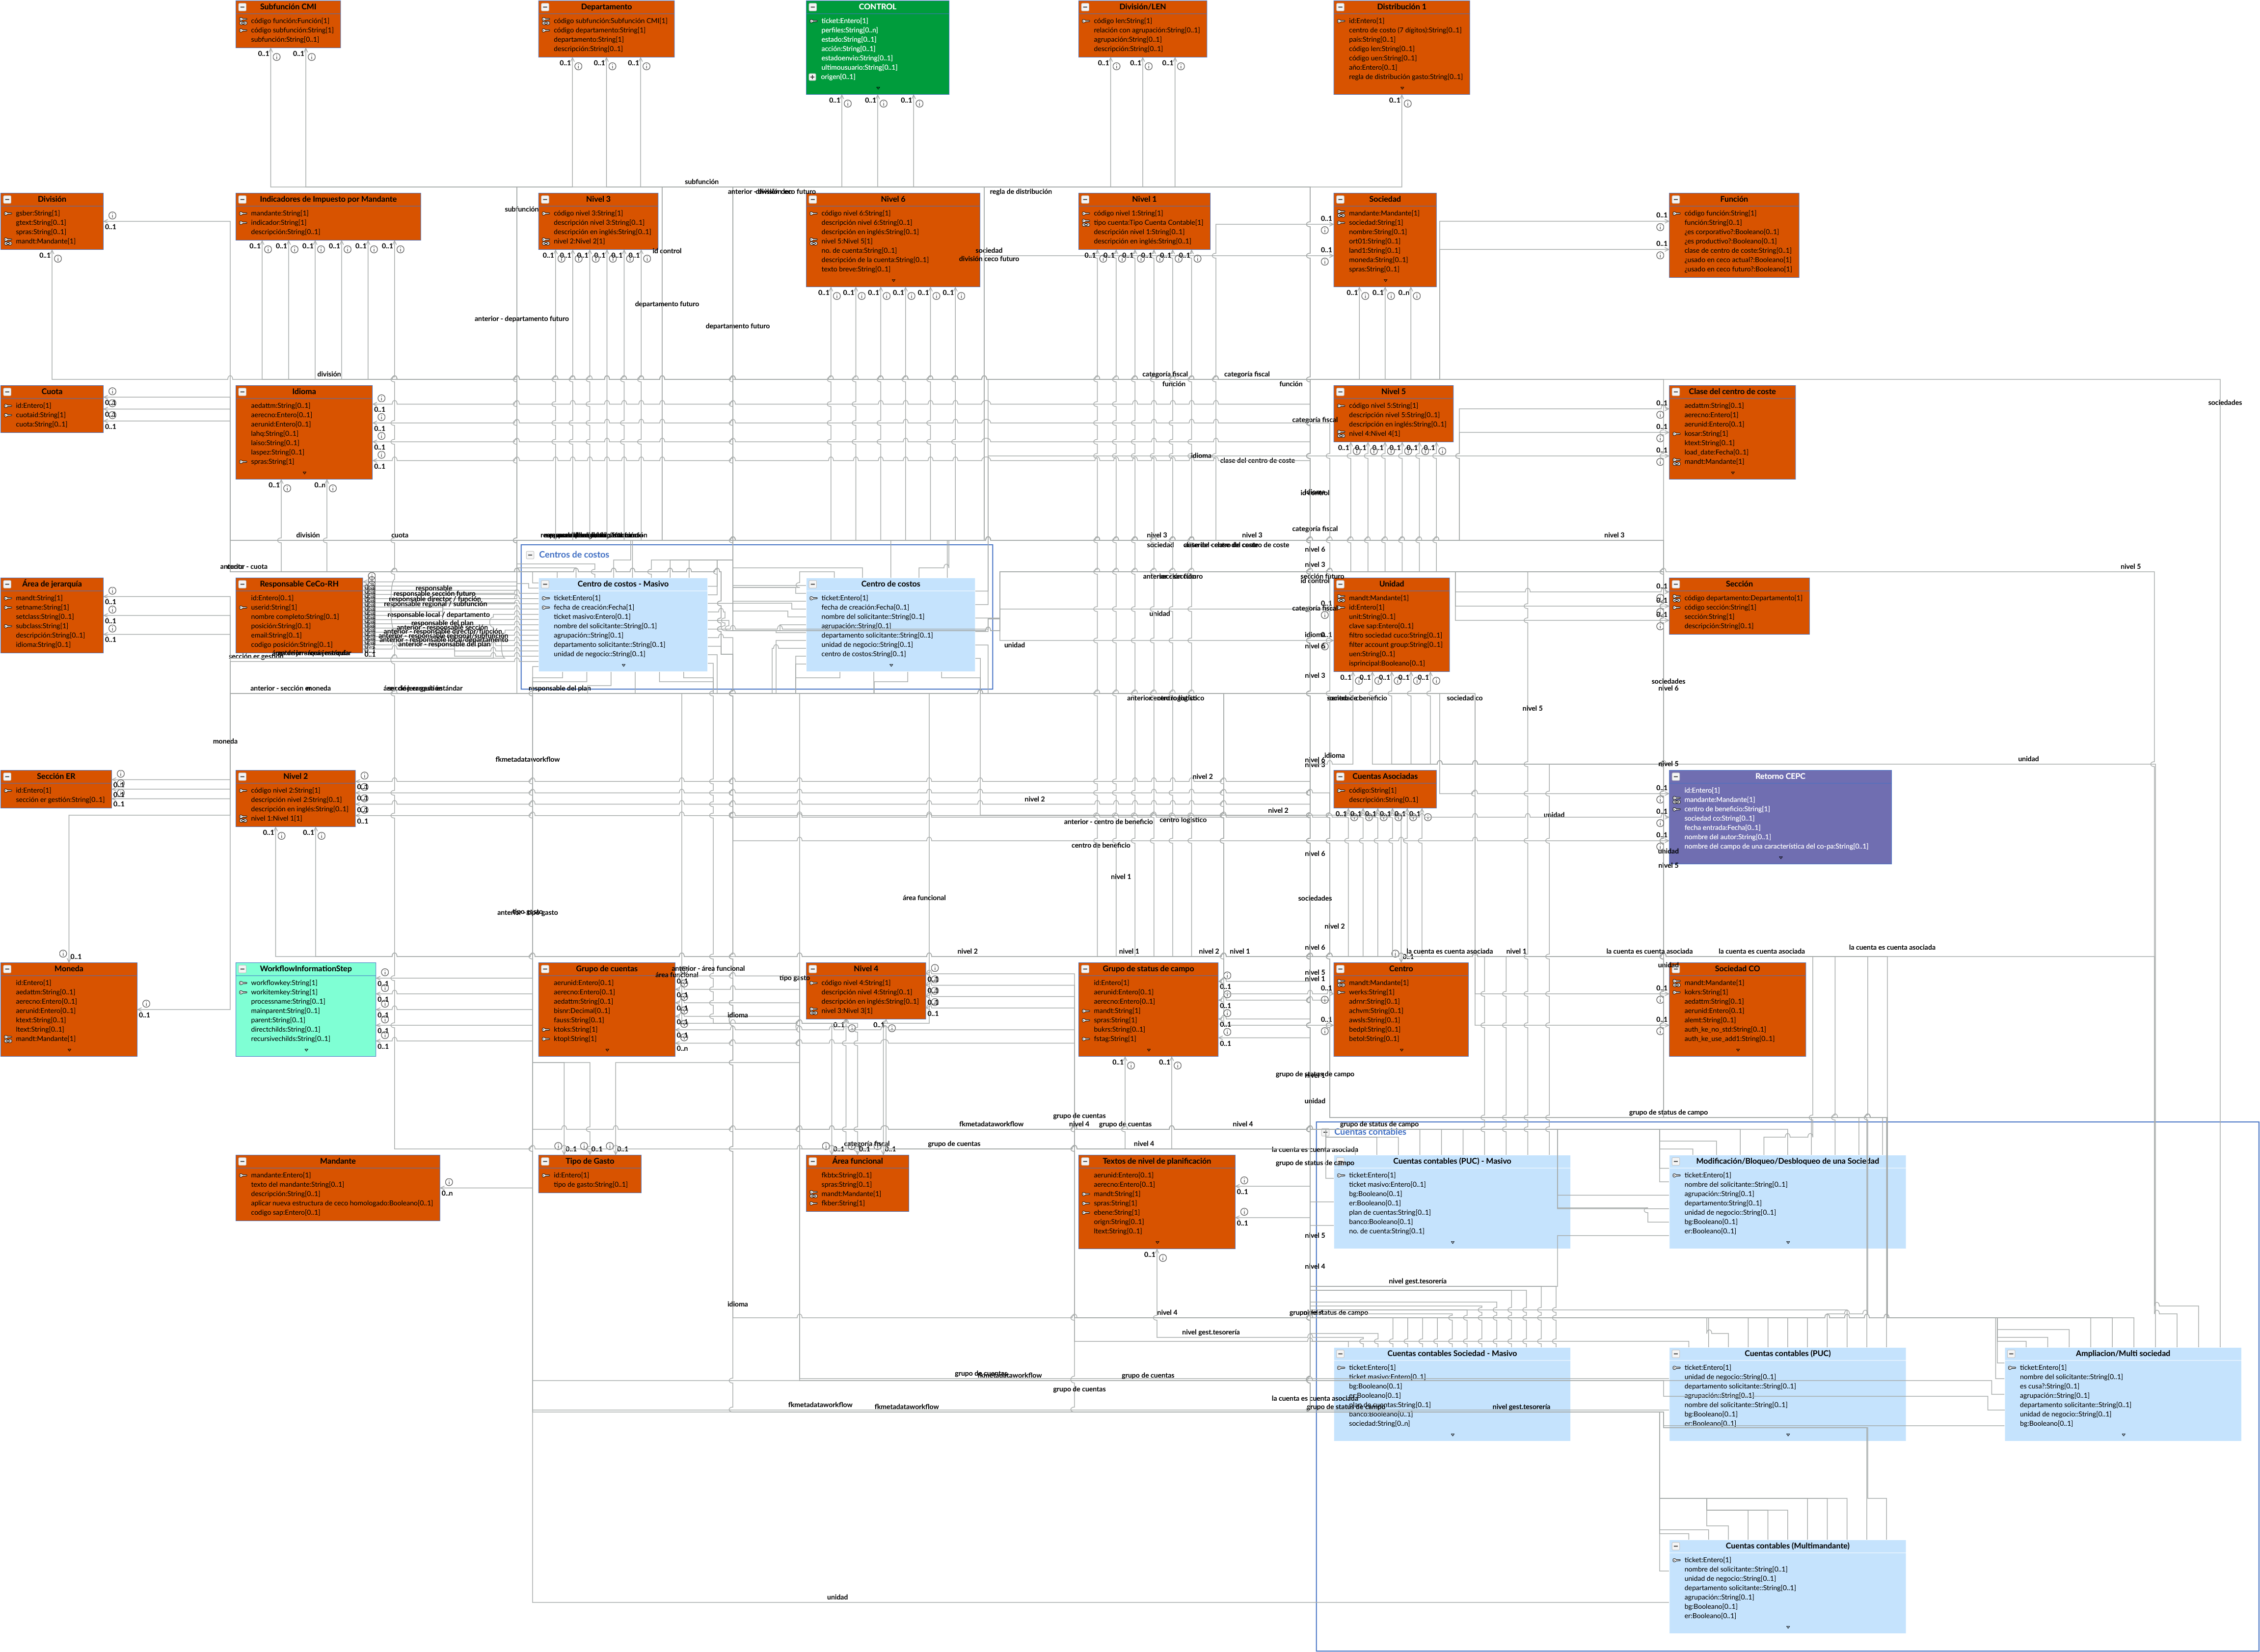
\includegraphics[width=0.8\textwidth]{ModeloDatos/ImagenesModelosDatos/TablasHistorico.png}
    \caption{Diagrama del modelo de datos de Histórico}
\end{figure}


\begin{quote}
  \textbf{Nota:} Para mejor calidad se adjuntan imágenes de los diagramas en el correo.
\end{quote}


%% ######### Carga Masiva

\subsection{[CA] Admin de Cargas Masivas}


Modelo encargado de administrar el proceso de cargas masivas.

\begin{enumerate}
    \item Configuración: Alineación de campos que harán referencia a tablas durante el proceso. 
    
    \item Carga:Tabla que contiene la información de donde se crearon los registros masivos de forma individual.

    \item Control: Tabla que contiene el control de estado de cada registro individual.

    \item Flujos: Listados de identificadores donde se configura la carga masiva.

    \item Pasos: Tabla que contiene los pasos a seguir al iniciar el proceso de carga masiva, depende de la tabla de Ruteo.

    \item Ruteo: Tabla que contiene las condicionales para iniciar y asignar variables a los flujos de trabajo de carga masiva.

    \item Histórico: Tabla que contiene el histórico transaccional del proceso de carga masiva. 

    \item Auxiliar: Tabla de respaldo donde se pueden colocar variables importantes a utilizar en los flujos de trabajo.
\end{enumerate}

\begin{figure}[H]
    \centering
    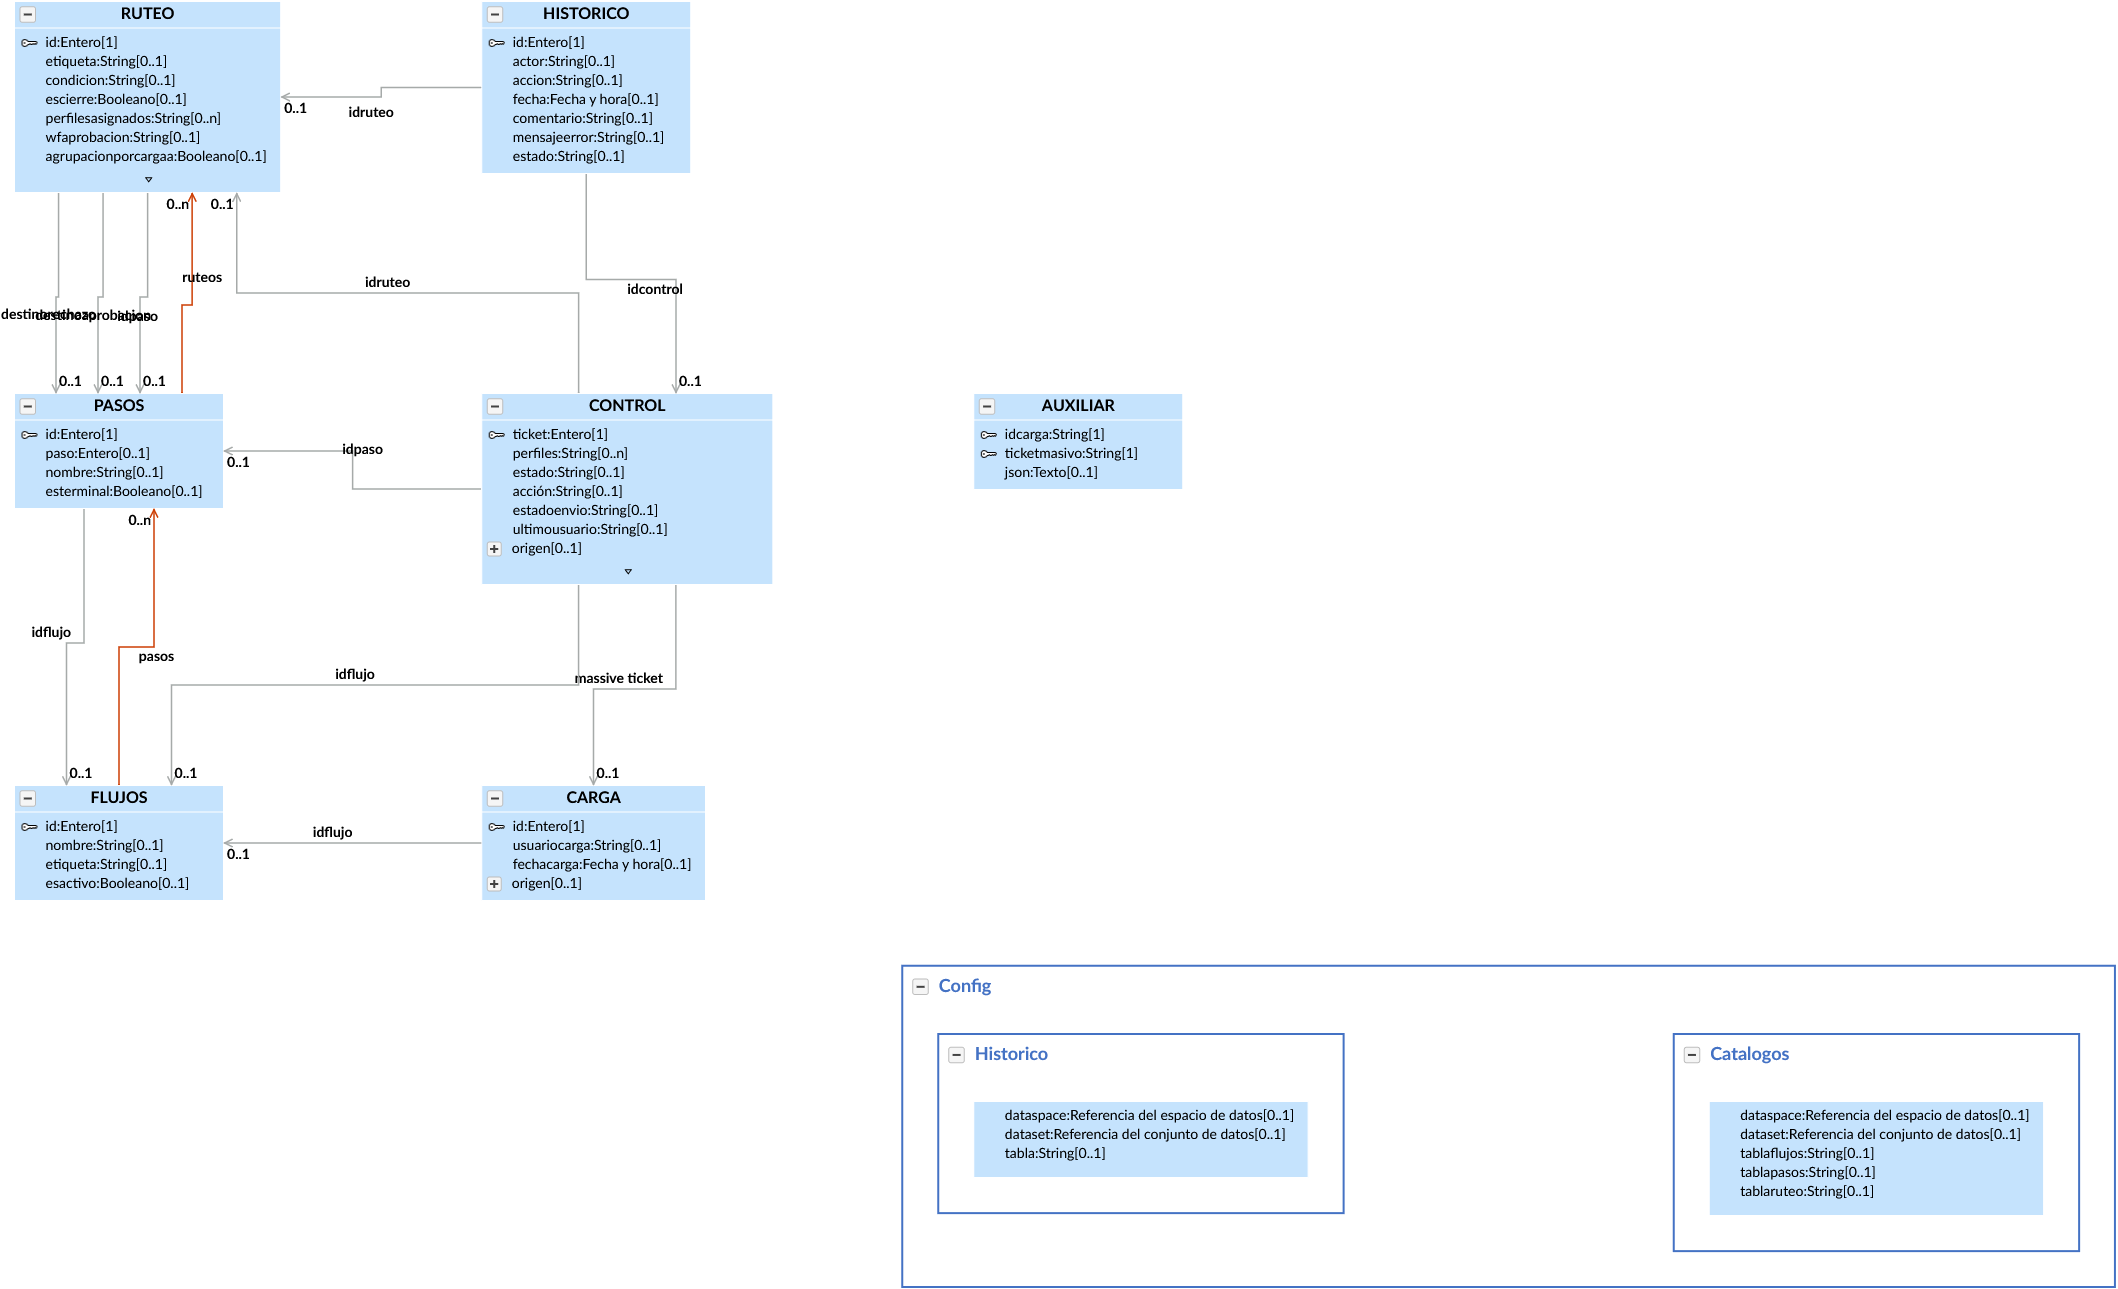
\includegraphics[width=0.8\textwidth]{ModeloDatos/ImagenesModelosDatos/CECO_MASIVO_T.png}
    \caption{Diagrama del modelo de datos de Carga Masiva}
\end{figure}


\begin{quote}
  \textbf{Nota:} Para mejor calidad se adjuntan imágenes de los diagramas en el correo.
\end{quote}

\subsection{Diagrama de modelo de datos}

Para visualizar el diagrama del modelo de datos, desde el modelo se accede a la opción de “Acciones”.

En el menú que se despliega, se selecciona la opción de “Visualización”, para posteriormente seleccionar “Mostrar modelo de datos”.

\begin{figure}[H]
    \centering
    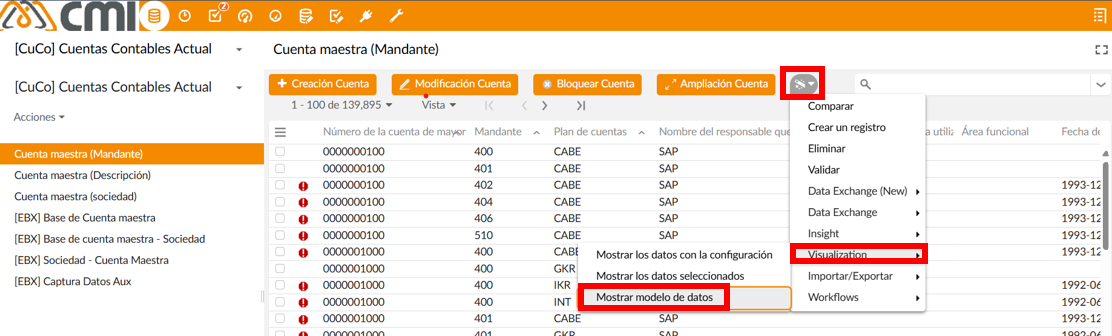
\includegraphics[width=0.8\textwidth]{ModeloDatos/ImagenesModelosDatos/DMD01.png}
    \caption{Pasos para acceder al diagrama de modelo de datos.}
\end{figure}

Una vez seleccionada la opción anterior, se visualizará el diagrama que compone al modelo de datos.

\begin{figure}[H]
    \centering
    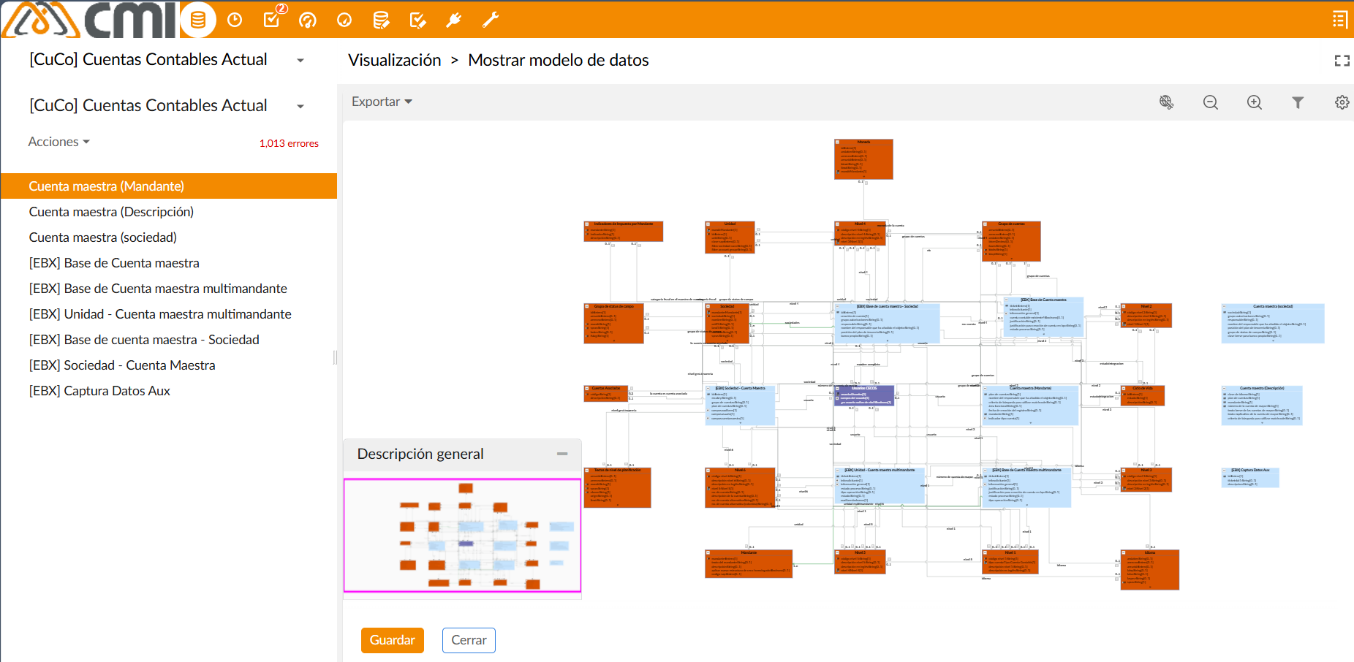
\includegraphics[width=0.8\textwidth]{ModeloDatos/ImagenesModelosDatos/DMD02.png}
    \caption{Visualización del diagrama del modelo de datos.}
\end{figure}

Dicho modelo se puede exportar, dando clic en la opción de “Export” y eligiendo el formato deseado para exportarlo.

\begin{figure}[H]
    \centering
    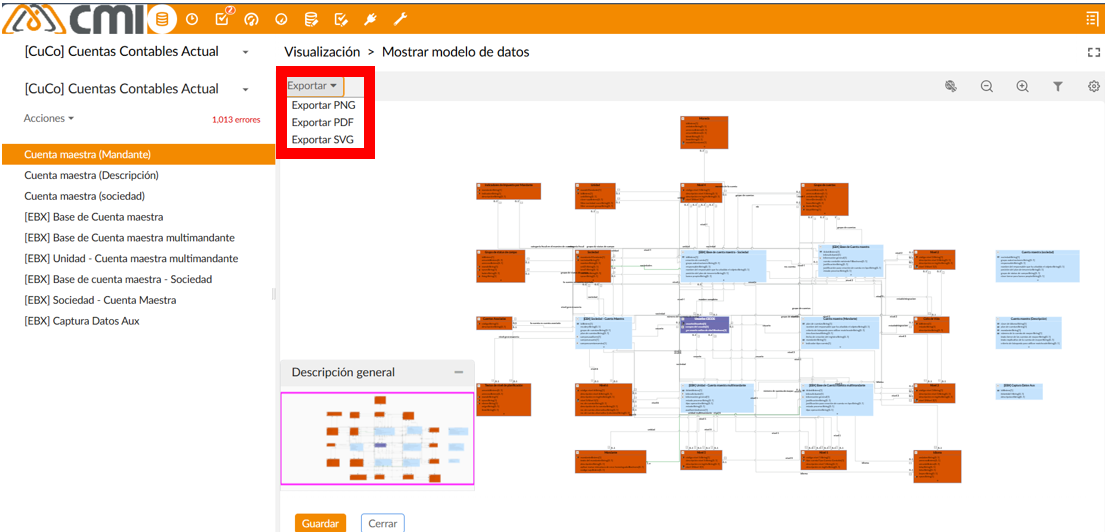
\includegraphics[width=0.8\textwidth]{ModeloDatos/ImagenesModelosDatos/DMD03.png}
    \caption{Exportar como imagen el diagrama del modelo de datos.}
\end{figure}







